\documentclass[slidestop,compress,mathserif]{beamer}
%\documentclass[slidestop,compress,mathserif,handout]{beamer}

%\documentclass[xcolor=dvipsnames,handout]{beamer}
%\documentclass[xcolor=dvipsnames]{beamer}

%\documentclass[handout]{beamer}

%%% To get rid of solutions on handouts:
\newcommand{\soln}[1]{\textit{\textcolor{darkGray}{#1}}}				% For slides
%\newcommand{\soln}[1]{ }	% For handouts

% to get pausing to work properly on slides
\newcommand{\hide}[1]{#1}	% For slides
%\newcommand{\hide}[1]{ }	% For handouts

%\newtheorem{defn}{Definition}

%\usepackage{multicol}
\usepackage{amsfonts}
%\usepackage[pdftex,dvipsnames]{color}
\usepackage{graphicx}
\usepackage{subfigure}
%\usepackage{picinpar}
\usepackage{pifont}
\usepackage{pgf,pgfarrows,pgfnodes}
%\usepackage{wasysym,manfnt,phaistos,empheq}
\usepackage[english]{babel}
\usepackage{pgfpages}
\usepackage{natbib}
\usepackage{hyperref}
\usepackage{multimedia}
%\usepackage{amsfonts,amstext,amssymb,amsbsy,amsopn,amsthm,eucal,latexsym,mathrsfs}
\usepackage{amsmath,amsfonts,amstext,amssymb,amsbsy,amsopn,amsthm,eucal,latexsym,mathrsfs}
\usepackage{ulem}
\usepackage{setspace}
\usepackage{array}
%\usepackage{rotating}
\usepackage{multirow}
\usepackage{verbatim}
\usepackage{multicol}

\setbeamertemplate{navigation symbols}{}

%\usepackage{tikz}
%\usetikzlibrary{arrows,shapes,trees,backgrounds}


%\setbeameroption{show notes on second screen}
%\setbeameroption{show notes}
%\setbeameroption{show only notes}

\definecolor{links}{HTML}{2A1B81}
\hypersetup{colorlinks,linkcolor=,urlcolor=links}

\newtheorem*{principle}{Inscrutibility Principle}
\newtheorem*{punchline}{Punch Line}
\newtheorem{defn}{Definition}

\definecolor{Scarlet}{RGB}{140,17,17}
\definecolor{VassarRed}{RGB}{128,0,0}

% "dinglist" environment
  \renewenvironment{dinglist}[2][blue]
  {\begin{list}{\textcolor{blue}{\ding{#2}}}{}}{\end{list}}
  % Symbol definitions for these lists
  \newcommand{\DingListSymbolA}{43}
  \newcommand{\DingListSymbolB}{243}
  \newcommand{\DingListSymbolC}{224}
  \newcommand{\DingListSymbolD}{219}
  \newcommand{\DingListSymbolCheck}{52}
  \newcommand{\DingListSymbolCross}{56}


  \newenvironment{ballotenv}
{\only{%
\setbeamertemplate{itemize item}{\ding{45}}%
\setbeamertemplate{itemize subitem}{\ding{46}}%
\setbeamertemplate{itemize subsubitem}{\ding{46}}}} {}
\setbeamertemplate{itemize item}{\ding{49}}
\setbeamertemplate{itemize subitem}{\ding{47}}
\setbeamertemplate{itemize subsubitem}{\ding{47}}


%User defined colors: See colors section
\xdefinecolor{oiBlue}{rgb}{0.15, 0.35, 0.55}
\xdefinecolor{gray}{rgb}{0.5, 0.5, 0.5}
\xdefinecolor{darkGray}{rgb}{0.3, 0.3, 0.3}
\xdefinecolor{darkerGray}{rgb}{0.2, 0.2, 0.2}
\xdefinecolor{rubineRed}{rgb}{0.89,0,0.30}
\xdefinecolor{linkCol}{rgb}{0.11,0.49,0.95}	
\xdefinecolor{irishGreen}{rgb}{0,0.60,0}	
\xdefinecolor{darkturquoise}{rgb}{0.44, 0.58, 0.86}
\definecolor{lightGreen}{rgb}{0.533,0.765,0.42}
\xdefinecolor{Regalia}{HTML}{522D80}
\xdefinecolor{ClemsonOrange}{HTML}{EA6A20}

\definecolor{duke@LightGrey}{RGB}{200,200,200}\definecolor{DarkGreen}{RGB}{0,100,0}
\definecolor{Oranges}{RGB}{255,127,0}
\definecolor{LightGray}{RGB}{211,211,211}

%\setbeamertemplate{footline}{%
%  \raisebox{5pt}{\makebox[\paperwidth]{\hfill\makebox[10pt]{\scriptsize\insertframenumber}}}}

\setbeamercolor{equation background}{fg=black,bg=duke@LightGrey}
  % Boxed equation
  \newcommand{\eqbox}[2][0.6]{%
  \centerline{
  \begin{beamerboxesrounded}[lower=equation background,width=#1\hsize,shadow=true]{}
\parbox{#1\hsize}{%
      \[
        \textcolor{black} {#2}
      \]}
  \end{beamerboxesrounded}
}}

\AtBeginSection[] {
  \begin{frame}<beamer>\frametitle{Outline}
    \tableofcontents[currentsection,hideothersubsections]
  \end{frame}
}
%
%
%\AtBeginSubsection[] {
%  \begin{frame}<beamer>\frametitle{Outline}
%    \tableofcontents%[currentsection,currentsubsection]
%  \end{frame}
%}

%\usecolortheme[RGB={82,45,128}]{structure}
%\usecolortheme[RGB={162,80,22}]{structure}
\usecolortheme[RGB={128,0,0}]{structure}
\usetheme[secheader]{Boadilla}
%\usetheme[height=7mm]{Rochester}
%\usetheme{Copenhagen}
%\usetheme{Antibes}
%\usecolortheme{seahorse}
%\usecolortheme{crane}
%\usecolortheme{rose}
%\usefonttheme[onlylarge]{structurebold}
%\usefonttheme[onlymath]{serif}



\def\diag{{\rm diag}}


\def\E{\mathbb{E}}
\def\Prob{\mathbb{P}}
\def\argmin{{\rm argmin}}
\def\argmax{{\rm argmax}}
\def\Def{\stackrel{def}{=}}


\newtheorem{assumption}{Assumptions}
\newtheorem*{proposition}{Proposition}
\newtheorem*{remark}{Remark}



%\setbeamercolor{disc title}{bg=oiBlue!40!white!60,fg=blue}
\setbeamercolor{disc body}{bg= Regalia!20!white!80,fg= Regalia!80!black!90}

\setbeamercolor{clicker ungraded title}{bg=irishGreen!80!white!50,fg=irishGreen!30!black!90}
\setbeamercolor{clicker ungraded body}{bg=irishGreen!20!white!80,fg=irishGreen!30!black!90}

\setbeamercolor{clicker review title}{bg=gray!80!white!80,fg=oiBlue!80!black!90}
\setbeamercolor{clicker review body}{bg=gray!30!white!90,fg=oiBlue!80!black!90}

\setbeamercolor{code body}{bg=gray!20!white!80,fg=black}


% Custom commands
\newcommand{\degree}{\ensuremath{^\circ}}
\newcommand{\Note}[1]{
\rule{2.5cm}{0.25pt} \\ \textit{\scriptsize {\textcolor{rubineRed}{Note:} \textcolor{gray}{#1}}}}
\newcommand{\ct}[1]{
\vfill
{\tiny #1}}
\newcommand{\Remember}[1]{\textit{\scriptsize{\textcolor{orange}{Remember:} \textcolor{gray}{#1}}}}
\newcommand{\red}[1]{\textit{\textcolor{rubineRed}{#1}}}
\newcommand{\pink}[1]{\textit{\textcolor{rubineRed!90!white!50}{#1}}}
\newcommand{\green}[1]{\textit{\textcolor{irishGreen}{#1}}}
\newcommand{\webURL}[1]{\urlstyle{same}\textit{\textcolor{linkCol}{\url{#1}}} }
\newcommand{\webLink}[2]{\href{#1}{\textcolor{linkCol}{{#2}}}}
\newcommand{\mail}[1]{\href{mailto:#1}{\textit{\textcolor{linkCol}{#1}}}}
\newcommand{\hl}[1]{\textit{\textcolor{oiBlue}{#1}}}
\newcommand{\hlGr}[1]{\textit{\textcolor{lightGreen}{#1}}}
\newcommand{\mathhl}[1]{\textcolor{oiBlue}{\ensuremath{#1}}}
\newcommand{\ex}[1]{\textcolor{blue}{{{\small (#1)}}}}
\newcommand{\disc}[1]{
\begin{beamerboxesrounded}[shadow = true, lower = disc body, upper = disc title]{}
#1
\end{beamerboxesrounded}
}

\newcommand{\cl}[1]{
\begin{beamerboxesrounded}[shadow = true, lower = clicker ungraded body, upper = clicker ungraded title]{Question}
$\:$ \\
#1
\end{beamerboxesrounded}
}

\newcommand{\clR}[1]{
\begin{beamerboxesrounded}[shadow = true, lower = clicker review body, upper = clicker review title]{\red{Review question} }
$\:$ \\
#1
\end{beamerboxesrounded}
}

\newcommand{\formula}[2]{
\begin{beamerboxesrounded}[shadow = true, lower = white, upper = clicker review body]{#1}
#2
\end{beamerboxesrounded}
$\:$ \\
}

\newenvironment{twocol}[4]{
\begin{columns}[c]
\column{#1\textwidth}
#3
\column{#2\textwidth}
#4
\end{columns}
}


\newenvironment{slot}[2]{
\begin{array}{c}
\underline{#1} \\
#2
\end{array}
}

\newcommand{\pr}[1]{
\left( #1 \right)
}

\newcommand{\solnMult}[1]{
\item[] \vspace{-0.59cm}
\only<beamer| beamer:1>{\item #1}
\soln{\only<2->{\item \red{#1}}}
}

%\newcommand{\codechunk}[1]{
%\begin{beamerboxesrounded}[shadow = true, lower = code body]{}
%{\small #1}
%\end{beamerboxesrounded}
%}

% Change margin

\newenvironment{changemargin}[2]{%
\begin{list}{}{%
\setlength{\topsep}{0pt}%
\setlength{\leftmargin}{#1}%
\setlength{\rightmargin}{#2}%
\setlength{\listparindent}{\parindent}%
\setlength{\itemindent}{\parindent}%
\setlength{\parsep}{\parskip}%
}%
\item[]}{\end{list}}

% Footnote

\long\def\symbolfootnote[#1]#2{\begingroup%
\def\thefootnote{\fnsymbol{footnote}}\footnote[#1]{#2}\endgroup}

% Commands from the book
\newenvironment{data}[1]{\texttt{#1}}{}
\newenvironment{var}[1]{\texttt{#1}}{}
\newenvironment{resp}[1]{\texttt{#1}}{}






%%%%%%%%%%%%%%%%%%%%%%%%%%%%%%%%%%%%%%%%%%%%%%%%%%%%%%%%%%%%%%%%%%%%%%%%%%%%%%%%%%%%%%%%%%%%%%%

\title[Chapter 2]{Chapter 2}
\subtitle{Axioms of Probability}

%%%%%%%%%%%%%%%%%%%%%%%%%%%%%%%%%%%%%%%%%%%%%%%%%%%%%%%%%%%%%%%%%%%%%%%%%%%%%%%%%%%%%%%%%%%%%%%


\author[Jingchen (Monika) Hu]
{Jingchen (Monika) Hu}

\institute[Vassar]
{Vassar College}


\date[MATH 241]
{MATH 241}


\subject{MATH 241}



\begin{document}




%%%%%%%%%%%%%%%%%%%%%

% Title Page

\begin{frame}%[plain]
\titlepage
\end{frame}

%%%%%%%%%%%%%%%%%%%%%%
%\addtocounter{framenumber}{-1}
%
%\begin{frame}\frametitle{Annoucement}
%
%\begin{itemize}
%\item HW1: \red{due now}
%\item HW2: \red{due Tuesday, Sept 9th}
%\end{itemize}
%
%\begin{itemize}
%\item Quiz1: today
%\end{itemize}
%
%\end{frame}
%


%%%%%%%%%%%%%%%%%%%%%%%%%%%%%%%%%%%%%%%%%%
\section{Sample space and events}
%%%%%%%%%%%%%%%%%%%%%%%%%%%%%%%%%%%%%%%%%%
\begin{frame}\frametitle{Sample space}

\begin{defn}
A sample space $S$ is the set of all possible outcomes
of an experiment.
\end{defn}

\cl{Chapter 2 Problem 5: A system is composed of 5 components, each of which is either working or failed. Consider an experiment that consists of observing the status of each component, and let the outcome of the experiment be given by the vector $(x_1, x_2, x_3, x_4, x_5)$, where $x_i$ is equal to 1 if component $i$ is working and is equal to 0 if component $i$ is failed. \\

(a) How many outcomes are in the sample space of this experiment?}

 

$$2^5$$

\end{frame}

%%%%%%%%%%%%%%%%%%%%%%%%%%%%%%%%%%%%%%%%%%
\begin{frame}\frametitle{An event}

\begin{defn}
An event $E$ is any subset of the sample space $S$.
\[E \subset S\]
\end{defn}

\begin{itemize}
\item Impossible event: empty set $\O \subset S$
\item $S \subset S$
\end{itemize}

\end{frame}



\begin{frame}

\cl{Chapter 2 Problem 5: A system is composed of 5 components, each of which is either working or failed. Consider an experiment that consists of observing the status of each component, and let the outcome of the experiment be given by the vector $(x_1, x_2, x_3, x_4, x_5)$, where $x_i$ is equal to 1 if component $i$ is working and is equal to 0 if component $i$ is failed. \\

(b) Suppose that the system will work if components 1 and 2 are both working, or if components 3 and 4 are both working, or if components 1, 3, and 5 are all working. Let $W$ be the event that the system will work. Specify all the outcomes in $W$.}

 

$$W = \{(1, 1, ?, ?, ?), (?, ?, 1, 1, ?), (1, ?, 1, ?, 1)\}$$

{\color{red}Watch out for duplicate outcomes!}
\end{frame}


\begin{frame}

\cl{Chapter 2 Problem 5: A system is composed of 5 components, each of which is either working or failed. Consider an experiment that consists of observing the status of each component, and let the outcome of the experiment be given by the vector $(x_1, x_2, x_3, x_4, x_5)$, where $x_i$ is equal to 1 if component $i$ is working and is equal to 0 if component $i$ is failed. \\

(c) Let $A$ be the event that components 4 and 5 are both failed. How many outcomes are contained in the event $A$?}

 

$$A = \{(?, ?, ?, 0, 0)\}$$

The number of outcomes in event $A$ is $2^3$.

\end{frame}


%%%%%%%%%%%%%%%%%%%%%%%%%%%%%%%%%%%%%%%%%%
\begin{frame}
\frametitle{Set theory}

Let $A, B$ be two events.

\begin{defn}

\begin{enumerate}
\item \textbf{Intersection} $A \cap B$:  implies the event that both $A$ and $B$ occur
\item \textbf{Union} $A \cup B$: implies the event that at least one of $A$ or $B$ occur
\item The {\bf complement} of an event $A$ denoted $A^c$ (also notated $A^{\prime}$ or $\bar{A}$):
$A^c = S \backslash A$ - the event that $A$ does not occur
\item $A \subset B$ implies that the occurrence of $A$ implies the occurrence of $B$
\end{enumerate}
\end{defn}

\underline{Venn diagram}

\end{frame}


\begin{frame}

\cl{Chapter 2 Problem 5: A system is composed of 5 components, each of which is either working or failed. Consider an experiment that consists of observing the status of each component, and let the outcome of the experiment be given by the vector $(x_1, x_2, x_3, x_4, x_5)$, where $x_i$ is equal to 1 if component $i$ is working and is equal to 0 if component $i$ is failed. Suppose that the system will work if components 1 and 2 are both working, or if components 3 and 4 are both working, or if components 1, 3, and 5 are all working. Let $W$ be the event that the system will work. Let $A$ be the event that components 4 and 5 are both failed. \\

(d) Write out all the outcomes in the event $A \cap W$.}


$$W = \{(1, 1, ?, ?, ?), (?, ?, 1, 1, ?), (1, ?, 1, ?, 1)\}, \,\,\, A = \{(?, ?, ?, 0, 0)\}$$

 

$$A \cap W = \{(1, 1, 0, 0, 0), (1, 1, 1, 0, 0)\}$$


\end{frame}


%%%%%%%%%%%%%%%%%%%%%%%%%%%%%%%%%%%%%%%%%%
\begin{frame}\frametitle{More set theory}

\begin{defn}
Two events $A$ and $B$ are {\bf mutually exclusive} or {\bf disjoint}
if they have no outcomes in common, i.e. $A\cap B=\O$.
\end{defn}

\vspace{.1in}
% 
%Being a Duke fan and a UNC Chapel Hill fan is mutually exclusive.



\end{frame}



%%%%%%%%%%%%%%%%%%%%%%%%%%%%%%%%%%%%%%%%%%
\begin{frame}\frametitle{Some rules}

\begin{enumerate}

\item Commutative laws
\[ A \cup B = B \cup A, \quad A \cap B = B \cap A \]
 

\item Associative laws
\[(A \cup B) \cup C = A \cup (B \cup C) \]
\[(A \cap B) \cap C = A \cap (B \cap C)\]
 

\item Distributive laws
\[(A \cup B) \cap C = (A \cap C) \cup (B \cap C)\]
\[(A \cap B) \cup C = (A \cup C) \cap (B \cup C)\]

\end{enumerate}


%\Note{Think of union as addition and intersection as multiplication: $(A+B)C = AC + BC$}


\end{frame}

%%%%%%%%%%%%%%%%%%%%%%%%%%%%%%%%%%%%%%%%%%
\begin{frame}\frametitle{DeMorgan's Laws}

\[(A \cup B)^c = A^c \cap B^c, \quad
(A \cap B)^c = A^c \cup B^c\]

 

\begin{itemize}
\item Outline of proof (to the first equation): two steps\\
Left $\subset$ Right $\Longleftrightarrow$ For any $x \in (A \cup B)^c$, then $x \in A^c \cap B^c$.\\
Right $\subset$ Left $\Longleftrightarrow$ For any $x \in A^c \cap B^c$, then $x \in (A \cup B)^c$.\\

 
\vspace{2.8cm}
\item DeMorgan's laws can be generalized to $n$ events $A_1, \ldots, A_n$:
\[
\left(\bigcup\limits_{i=1}^n  A_i \right)^c  =  \bigcap_{i=1}^n A_i^c, \quad
\left(\bigcap\limits_{i=1}^n  A_i \right)^c  =  \bigcup_{i=1}^n A_i^c
\]
\end{itemize}

 
\ct{\webURL{https://www.youtube.com/watch?v=oOx7FSzSav4}}


\end{frame}

%%%%%%%%%%%%%%%%%%%%%%%%%%%%%%%%%%%%%%%%%%
\begin{frame}\frametitle{Recap}

\begin{itemize}

\item Sample space $S$, event $E$
\item Set operations: intersection, union, complement, subset, disjoint/mutually exclusive
\item Rules: commutative, associative, distributive, DeMorgan's laws
\item Hint: Venn Diagram is helpful
\end{itemize}

\end{frame}


%%%%%%%%%%%%%%%%%%%%%%%%%%%%%%%%%%%%%%%%%%

%%%%%%%%%%%%%%%%%%%%%%
%\begin{frame}{Outline}
%%\tableofcontents[hideallsubsections,pausections]
%\tableofcontents[hideallsubsections]
%\end{frame}
%
%


%%%%%%%%%%%%%%%%%%%%%%%%%%%%%%%%%%%%%%%%%%
\section{Axioms of Probability}
%%%%%%%%%%%%%%%%%%%%%%%%%%%%%%%%%%%%%%%%%%


%%%%%%%%%%%%%%%%%%%%%%%%%%%%%%%%%%%%%%%%%%
%%%%%%%%%%%%%%%%%%%%%%%%%%%%%%%%%%%%%%%%%%
\begin{frame}\frametitle{Axioms of probability}

\vspace{-0.3cm}
\begin{defn}
Let $P$ be a function that assigns a nonnegative real number to each event $E$ of a sample space $S$.
We call $P$ a \hl{probability} if
 
\begin{enumerate}
\item Axiom 1: non-negative \[0 \leq P(E)  \leq 1\]
\vspace{-0.7cm}
 
\item Axiom 2: total one \[P(S) =  1\]
\vspace{-0.7cm}
 
\item Axiom 3: countable addition
\[P\left(\underset{i=1}{\overset{\infty}{\bigcup}} E_i\right) = \sum_{i=1}^\infty P(E_i) \text{,  if } E_i \cap E_j=\O \text{ for } i \neq j  \]
\end{enumerate}
\end{defn}
 
In particular, for $k$ {\bf disjoint} events $E_1, \ldots, E_k$,
\[P\left(\underset{i=1}{\overset{k}{\bigcup}} E_i\right) = \sum_{i=1}^k P(E_i)\]
\end{frame}

%%%%%%%%%%%%%%%%%%%%%%%%%%%%%%%%%%%%%%%%%%
%\begin{frame}\frametitle{Examples of probability}
%Based on the initial survey, for a randomly selected student from this class,
%\begin{itemize}
%\item $P(\text{female}) = 39\%$.
%\item $P(\text{math major}) = 42\%$.
%\item $P(\text{has a part time job}) = 42\%$.
%\item $P(\text{vegetarian}) = 3\%$.
%\end{itemize}
%
%\end{frame}

%%%%%%%%%%%%%%%%%%%%%%%%%%%%%%%%%%%%%%%%%%
\section{Some simple propositions}
%%%%%%%%%%%%%%%%%%%%%%%%%%%%%%%%%%%%%%%%%%
\begin{frame}\frametitle{Propositions}
\begin{dinglist}{\DingListSymbolA}
\item Complement Rule:
\[P(A^c) = 1-P(A)\]
\end{dinglist}

\begin{itemize}
\item $ P(\O) = 0 $
\end{itemize}

\begin{dinglist}{\DingListSymbolA}
\item Difference Rule:
\[  P(B \cap A^c) = P(B)-P(A) \text{, if } A \subseteq B \]
\end{dinglist}

\begin{itemize}
\item $ P(B) \geq P(A) \text{, if } A \subseteq B $
\end{itemize}

\begin{dinglist}{\DingListSymbolA}
\item Inclusion-Exclusion: two events $A, B$ (not necessarily disjoint)
  \[ P(A \cup B) = P(A) + P(B) - P(A \cap B) \]
\end{dinglist}
%\vspace{0.2cm}



\end{frame}



%%%%%%%%%%%%%%%%%%%%%%%%%%%%%%%%%%%%%%%%%%

\begin{frame}

\cl{What is the probability of drawing a jack or a red card from a well shuffled full deck?}
 
\begin{figure}
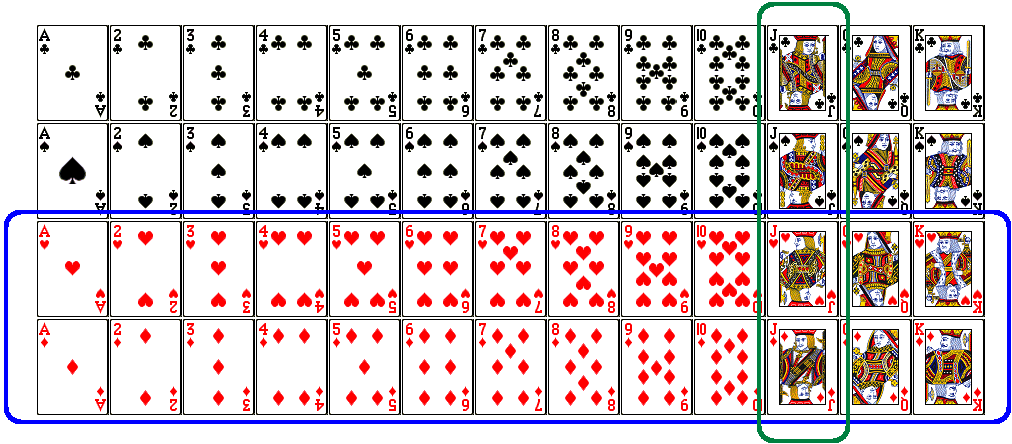
\includegraphics[width=0.7\textwidth]{figures/cards}
\end{figure}

\vspace{-0.75cm}

 
\begin{align*}
P(jack~or~red) &= P(jack) + P(red) - \red{$P(jack~and~red)$} \\
&= \frac{4}{52} + \frac{26}{52} - \frac{2}{52} = \frac{28}{52}
\end{align*}


\vfill

\ct{Figure from \webURL{http://www.milefoot.com/math/discrete/counting/cardfreq.htm}.}


\end{frame}


%%%%%%%%%%%%%%%%%%%%%%%%%%%%%%%%%%%%%%%%%%
\begin{frame}\frametitle{Propositions}
\begin{dinglist}{\DingListSymbolA}
\item Inclusion-Exclusion: three events $A, B, C$ (not necessarily disjoint)
  \begin{align*}
  P(A \cup B \cup C) = & P(A) + P(B) + P(C) - P(A \cap B) \\
                  		  & - P(A \cap C)  - P(B \cap C) + P(A \cap B \cap C)
  \end{align*}
\end{dinglist}
\begin{center}
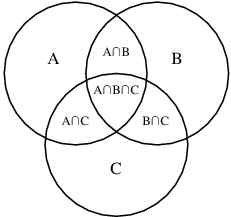
\includegraphics[width=0.45\textwidth]{Figures/venn.png}
\end{center}


\end{frame}


%%%%%%%%%%%%%%%%%%%%%%%%%%%%%%%%%%%%%%%%%%
\begin{frame}%\frametitle{Inclusion-Exclusion example}

\cl{{\footnotesize{Suppose that for a randomly selected student in a probability class,
\begin{itemize}
\item $P(\text{live Eastern Time Zone at home}) = 63\%$, $P(\text{senior}) = 41\%$, $P(\text{brown eye color}) = 55\%$.
\item $P(\text{live Eastern Time Zone at home and senior}) = 31\%$, $P(\text{live Eastern Time Zone at home and brown eye color}) = 33\%$,
$P(\text{senior and brown eye color}) = 24\%$
\item $P(\text{live Eastern Time Zone at home and senior and brown eye color}) = 18\%$
\end{itemize}
Find the probability that a student is either live Eastern Time Zone at home, a senior or having brown eye color.
}}
}
 
{\footnotesize{
\begin{enumerate}
\item \underline{Conditions}: Event $A = \{\text{live Eastern Time Zone at home}\}$, $B = \{ \text{senior} \}$, $C = \{ \text{brown eye color} \}$,
 \item \underline{Question}: find $P(A \cup B \cup C)$. 
\item \underline{Formula}: inclusion-exclusion
  \begin{align*}
  P(A \cup B \cup C) = & P(A) + P(B) + P(C) - P(A \cap B) \\
                  		  & - P(A \cap C)  - P(B \cap C) + P(A \cap B \cap C)\\
		  & = 0.63 + 0.41 + 0.55 - 0.31 - 0.33 - 0.24 + 0.18 = 0.89
  \end{align*}


\end{enumerate}

}}
\end{frame}


%%%%%%%%%%%%%%%%%%%%%%%%%%%%%%%%%%%%%%%%%%
\begin{frame}\frametitle{Recap}

Three axioms of probability $P$
\begin{enumerate}
\item $0 \leq P(E)  \leq 1$
\item $P(S) =  1$
\item $P\left(\underset{i=1}{\overset{\infty}{\cup}} E_i\right) = \sum_{i=1}^\infty P(E_i) \text{,  if } E_i \cap E_j=\emptyset \text{ for } i \neq j$
\end{enumerate}

 
Propositions of probability
\begin{itemize}
\item $P(A^c) = 1-P(A)$
\item $P(B \cap A^c) = P(B)-P(A) \text{, if } A \subseteq B$
\item $P(A \cup B) = P(A) + P(B) - P(A \cap B)$
\item $P(A \cup B \cup C) = P(A) + P(B) + P(C) - P(A \cap B) - P(A \cap C)  - P(B \cap C) + P(A \cap B \cap C)$
\end{itemize}


\end{frame}

%%%%%%%%%%%%%%%%%%%%%
%\begin{frame}{Outline}
%%\tableofcontents[hideallsubsections,pausections]
%\tableofcontents[hideallsubsections]
%\end{frame}




%%%%%%%%%%%%%%%%%%%%%%%%%%%%%%%%%%%%%%%%%%
\section{Sample spaces with equally likely outcomes}
%%%%%%%%%%%%%%%%%%%%%%%%%%%%%%%%%%%%%%%%%%
\begin{frame}\frametitle{Sample spaces with equally likely outcomes}
\begin{dinglist}{\DingListSymbolA}
\item Suppose a sample space has $N$ equally likely outcomes $\{1\}, \ldots, \{N\}$, then
\[
S = \{1\} \cup \ldots \cup \{N\}
\]
Disjointness gives
\[
1 = P(S) = P(\{1\}) + \ldots + P(\{N\}) = NP(\{i\}),
\]
so for each $1\leq i \leq N$,
\[
P(\{i\}) = \frac{1}{N}
\]

\uncover<2->{
\item For event $E$ in a sample space $S$ with equally likely outcomes,
\[P(E) = \frac{\#(E)}{\#(S)}  \] %=  \sum_i \frac{1_{ \omega_i \in E}}{\#(S)}\]

Notation: \\
\vspace{2mm} \hspace{2mm} Cardinality - $\#(E) =  \text{number of elements in set } E$\\
}
\end{dinglist}
\end{frame}




%%%%%%%%%%%%%%%%%%%%%%%%%%%%%%%%%%%%%%%%%%

\begin{frame}%\frametitle{TBD}

\cl{Two fair four-sided dice are rolled. Two events:
\vspace{-0.4cm}
\begin{align*}
A & = \{ \text{sum of two rolls is 5} \}\\
B & = \{ \text{minimum roll is 2} \}
\end{align*}
\vspace{-0.8cm}
\begin{enumerate}
\item Compute $P(A)$ and $P(B)$
\item Compute $P(A \cup B)$
\end{enumerate}
}

 
%\vspace{0.3cm}

\twocol{0.4}{0.6}
{
Hint: sample space
\begin{center}
\begin{tabular}{cccc}
1,1 & 1,2 & 1,3 & 1,4 \\
2,1 & 2,2 & 2,3 & 2,4 \\
3,1 & 3,2 & 3,3 & 3,4 \\
4,1 & 4,2 & 4,3 & 4,4 \\
\end{tabular}
\end{center}
}
{
 
\begin{enumerate}
\item
$P(A)  = \frac{4}{16}$, $P(B)  = \frac{5}{16}$
 
\item
\begin{align*}
P(A \cup B) & = P(A) + P(B) - P(A \cap B)\\
		  & = \frac{4}{16} + \frac{5}{16} - \frac{2}{16} = \frac{7}{16}\\
\end{align*}
\end{enumerate}
}
\end{frame}

%%%%%%%%%%%%%%%%%%%%%%%%%%%%%%%%%%%%%%%%%%

%%%%%%%%%%%%%%%%%%%%%%%%%%%%%%%%%%%%%%%%%%
%
%\begin{frame}
%\frametitle{$\log$ makes everything better}
%
%Remember:
%{\footnotesize
%\begin{align*}
%\log(XY) &= \log(X) + \log(Y)\\
%\log(X/Y) &= \log(X) - \log(Y)\\
%\log(X^b) &= b\log(X)
%\end{align*}
%}
% 
%\begin{itemize}
%\item Gamma function
%\[ \Gamma(n) = \int_0^\infty t^{n-1}e^{-t} dt\]
% 
%\item When $n$ is a positive integer,
%\[
%\Gamma(n+1) = n!
%\]
% 
%\item Most often a math library (include R) implement \texttt{gamma} and \texttt{lgamma}
%\end{itemize}
%
%\end{frame}
%

%%%%%%%%%%%%%%%%%%%%%%%%%%%%%%%%%%%%%%%%%%
\begin{frame}[fragile]\frametitle{Birthday problem (cont.)}

%\scriptsize{

\cl{For a class of 30 students (i.e. $n = 30$), $P(\text{no match}) = 29.4\%$.
What is the chance of at least a tie in birthdays among these 30 students?}
 
\[
P(\text{at least a tie}) = 1 - P(\text{no tie}) = 1 - 0.294 = 0.706
\]

% 
%We have a tie actually! \\
%Two students in this class have birthday on April 19.
\end{frame}
%%%%%%%%%%%%%%%%%%%%%%%%%%%%%%%%%%%%%%%%%%%
%\begin{frame}%[fragile]\frametitle{ (5 cards)}
%\disc{Example: in a poker hand, what's the probability of getting one pair?}
% 
%Equally likely outcomes!
%\[
%P(\text{one pair}) = \frac{\#(\text{one pair among 5 cards})}{\#(\text{all possible combanions})}
%\]
%
% 
%\begin{center}
%\begin{tabular}{ccccc}
%\underline{\hspace{1cm}} & \underline{\hspace{1cm}} & \underline{\hspace{1cm}} & \underline{\hspace{1cm}} & \underline{\hspace{1cm}} \\
%a & a & b & c & d\\
%\end{tabular}
%\end{center}
%
% 
%Order doesn't matter! Count the number of combinations.
%
%\[\#(\text{one pair})  = {13 \choose 1}{4 \choose 2}{12 \choose 3}{4 \choose 1}{4 \choose 1}{4 \choose 1}\]
%\[\#(\text{poker hand})  = {52 \choose 5}\]
%
%
%\[
%P(\text{one pair})  = \frac{\#(\text{one pair}) }
%				 {\#(\text{poker hand})} = 0.42
%\]
%
%
%\end{frame}
%
%
%%%%%%%%%%%%%%%%%%%%%%%%%%%%%%%%%%%%%%%%%%%
%%\begin{frame}\frametitle{How many ways of getting one pair?}
%%
%%\begin{center}
%%\begin{tabular}{ccccc}
%%\underline{\hspace{1cm}} & \underline{\hspace{1cm}} & \underline{\hspace{1cm}} & \underline{\hspace{1cm}} & \underline{\hspace{1cm}} \\
%%a & a & b & c & d\\
%%\end{tabular}
%%\end{center}
%%
%%\[
%%\#(\text{one pair}) = {13 \choose 1}{4 \choose 2}{12 \choose 3}{4 \choose 1}{4 \choose 1}{4 \choose 1}
%%\]
%%
%% 
%%
%%Common mistakes
%%\vspace{0.3cm}
%%\begin{itemize}
%%\item
%%$\#(\text{one pair}) ={13 \choose 1}{12 \choose 3}$   \hspace{1cm} \red{4 suits}
%% 
%%\item
%%$\#(\text{one pair}) ={13 \choose 1}{4 \choose 2} \times {12 \choose 1}{4 \choose 1}\times{11 \choose 1}{4 \choose 1}\times{10 \choose 1}{4 \choose 1}$\\
%%   \red{The order among \{b, c, d\} does not matter.}
%%\item
%%$\#(\text{one pair}) ={13 \choose 4}{4 \choose 2}{4 \choose 1}{4 \choose 1}{4 \choose 1}$\\
%%   \red{a is not exchangeable with b (or c or d).\\ \{aabcd\} and \{bbacd\} are different outcomes.}
%%
%%
%%\end{itemize}
%%
%%\end{frame}
%
%%%%%%%%%%%%%%%%%%%%%%%%%%%%%%%%%%%%%%%%%%%
%\begin{frame}[fragile]\frametitle{Poker hands (5 cards)}
%\disc{What's the probability of getting two pairs?}
%
%\begin{center}
%\begin{tabular}{ccccc}
%\underline{\hspace{1cm}} & \underline{\hspace{1cm}} & \underline{\hspace{1cm}} & \underline{\hspace{1cm}} & \underline{\hspace{1cm}} \\
%a & a & b & b & c\\
%\end{tabular}
%\end{center}
%
% 
%Order doesn't matter! Count the number of combinations.
%
%\[\#(\text{2 pairs})  = {13 \choose 2}{4 \choose 2}{4 \choose 2}{11 \choose 1}{4 \choose 1}\]
%\[\#(\text{poker hand})  = {52 \choose 5}\]
%
%
%\[
%P(\text{2 pairs})  = \frac{\#(\text{2 pairs}) }
%				 {\#(\text{poker hand})} = 0.048
%\]
%
%
%
%% 
%%\[
%%P(\text{2 pairs})  = \frac{{13 \choose 2}{4 \choose 2}{4 \choose 2}{11 \choose 1}{4 \choose 1}}
%%				 {{52 \choose 5}} = 0.047539
%%\]
%%
%% 
%%
%%\disc{What's the probability of getting 3 of a kind?}
%%
%%\begin{center}
%%\begin{tabular}{ccccc}
%%\underline{\hspace{1cm}} & \underline{\hspace{1cm}} & \underline{\hspace{1cm}} & \underline{\hspace{1cm}} & \underline{\hspace{1cm}} \\
%%a & a & a & b & c\\
%%\end{tabular}
%%\end{center}
%%
%% 
%%\[
%%P(\text{3 of a kind})  = \frac{{13 \choose 1}{4 \choose 3}{12 \choose 2}{4 \choose 1}{4 \choose 1}}
%%				 {{52 \choose 5}} = 0.021128
%%\]
%
%\end{frame}
%
%
%%%%%%%%%%%%%%%%%%%%%%%%%%%%%%%%%%%%%%%%%%%%
%%\begin{frame}[fragile]\frametitle{Poker hands (5 cards)}
%%\disc{What's the probability of getting a full house?}
%%
%%\begin{center}
%%\begin{tabular}{ccccc}
%%\underline{\hspace{1cm}} & \underline{\hspace{1cm}} & \underline{\hspace{1cm}} & \underline{\hspace{1cm}} & \underline{\hspace{1cm}} \\
%%a & a & a & b & b\\
%%\end{tabular}
%%\end{center}
%%
%%
%% 
%%\[
%%P(\text{full house})  = \frac{{13 \choose 1}{4 \choose 3}{12 \choose 1}{4 \choose 2}}
%%				 {{52 \choose 5}} = 0.0014
%%\]
%%
%% 
%%
%%\disc{What's the probability of getting a flush?}
%%
%%\begin{center}
%%\begin{tabular}{ccccc}
%%\underline{\hspace{1cm}} & \underline{\hspace{1cm}} & \underline{\hspace{1cm}} & \underline{\hspace{1cm}} & \underline{\hspace{1cm}} \\
%%\end{tabular}
%%\end{center}
%%\begin{center}
%%\begin{tabular}{c}
%%from the same suit
%%\end{tabular}
%%\end{center}
%%
%% 
%%\[
%%P(\text{flush})  = \frac{{13 \choose 5}{4 \choose 1}}
%%				 {{52 \choose 5}} = 0.001981
%%\]
%%
%%\end{frame}
%%
%
%
%%%%%%%%%%%%%%%%%%%%%%%%%%%%%%%%%%%%%%%%%%

\begin{frame}
\cl{Randomly pair 4 keys \{a, b, c, d\} with 3 locks \{a, b, c\}. \\
Compute $P(\text{at least one match})$.}

\uncover<2->{
Let $A$ denote the event that lock $a$ and key $a$ matches. Similarly, $B, C$.
\begin{itemize}
\item $P(A) = $ \uncover<3->{$\frac{3 \times 2}{4 \times 3 \times 2}$}
\item $P(A \cap B) = \uncover<4->{\frac{2}{4 \times 3 \times 2}$}
\item $P(A \cap B \cap C) = \uncover<5->{\frac{1}{4 \times 3 \times 2}$}
\item $P(\text{at least one match})=P(A \cup B \cup C) =$
\uncover<6->{
\footnotesize{
\begin{align*}
& P(A) + P(B) + P(C) - P(A \cap B) - P(A \cap C)  - P(B \cap C) + P(A \cap B \cap C)\\
= & \frac{6}{24} \times 3 - \frac{2}{24} \times 3 + \frac{1}{24}  = \frac{13}{24}
\end{align*}
}
}
\end{itemize}
}


\end{frame}



%%%%%%%%%%%%%%%%%%%%%%%%%%%%%%%%%%%%%%%%%%
\begin{frame}\frametitle{Recap}

For event $E$ in a sample space $S$ with equally likely outcomes,
\[P(E) = \frac{\#(E)}{\#(S)}  \] %=  \sum_i \frac{1_{ \omega_i \in E}}{\#(S)}\]

\pause
\cl{In the game of bridge, the entire deck of 52 cards is dealt out to 4 players. What is the probability that one of the players receives all face cards?}
%\begin{enumerate}[(a)]
%\item $12!/{52 \choose 12}$
%\only<beamer| beamer:2>{\item $40 \times 4 / {52 \choose 13}$}
%\only<3>{\item \red{$40 \times 4 / {52 \choose 13}$}}
%%\solnMult{$40 \times 4 / {52 \choose 13}$}
%\item $40 \times 4 / {52 \choose 12}$
%\item $40  / {52 \choose 13}$
%\end{enumerate}
\pause
\[ \#(\text{Player A gets all face cards}) = {12 \choose 12} {52-12 \choose 1} = 40 \]
\[ P(\text{Player A gets all face cards}) = \frac{40}{{52 \choose 13}} \]
\[ P(\text{one player gets all face cards}) = 4 \times \frac{40}{{52 \choose 13}}\]


\end{frame}

%%%%%%%%%%%%%%%%%%%%%
%\begin{frame}{Outline}
%%\tableofcontents[hideallsubsections,pausections]
%\tableofcontents[hideallsubsections]
%\end{frame}



%%%%%%%%%%%%%%%%%%%%%%%%%%%%%%%%%%%%%%%%%%



%%%%%%%%%%%%%%%%%%%%%%%%%%%%%%%%%%%%%%%%%%


\end{document}
